% 梯形中位线定理：MN 连两腰中点，MN ∥ AD ∥ BC, MN=(a+b)/2
\documentclass[tikz,border=4pt]{standalone}
\usepackage{ctex}
\usepackage{amsmath}
\usetikzlibrary{calc, decorations.markings}
\begin{document}
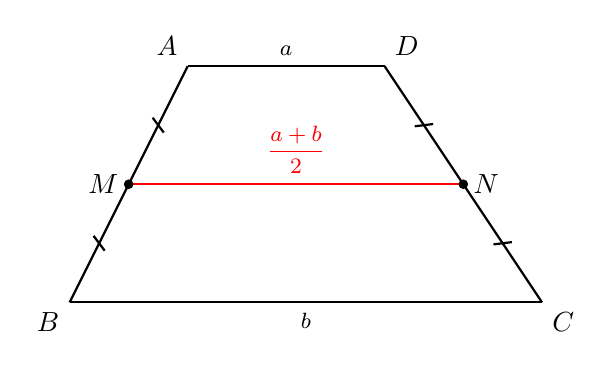
\begin{tikzpicture}[
  scale=1.0, thick,
  tickone/.style={postaction={decorate, decoration={markings,
    mark=at position 0.5 with {\draw (-1.5pt,-3pt) -- (1.5pt,3pt);}}}},
]
  \coordinate (A) at (1.5,3);
  \coordinate (D) at (4,3);
  \coordinate (B) at (0,0);
  \coordinate (C) at (6,0);
  \coordinate (M) at ($(A)!0.5!(B)$);
  \coordinate (N) at ($(D)!0.5!(C)$);

  \draw (A)--(D);
  \draw (B)--(C);
  \draw[tickone] (A)--(M); \draw[tickone] (M)--(B);
  \draw[tickone] (D)--(N); \draw[tickone] (N)--(C);

  \draw[red, thick] (M)--(N);

  \foreach \pt in {M,N} \filldraw (\pt) circle (1.3pt);

  \node[above left]  at (A) {$A$};
  \node[above right] at (D) {$D$};
  \node[below left]  at (B) {$B$};
  \node[below right] at (C) {$C$};
  \node[left]  at (M) {$M$};
  \node[right] at (N) {$N$};
  \node[above] at ($(A)!0.5!(D)$) {\footnotesize $a$};
  \node[below] at ($(B)!0.5!(C)$) {\footnotesize $b$};
  \node[above, red] at ($(M)!0.5!(N)$) {\footnotesize $\dfrac{a+b}{2}$};
\end{tikzpicture}
\end{document}
